\documentclass{article} % kind of document
\usepackage[utf8]{inputenc} %encoding of choice
\usepackage[american]{babel} %language of choice
\usepackage[p,osf]{cochineal}
\usepackage{fancyhdr} %for header
\usepackage{amsmath, tabu} %math mode
\usepackage{mathtools}
\usepackage{amssymb} %math symbols
\usepackage{dsfont} %specifically for the indicator function symbol
\usepackage{xcolor} %to color text
\usepackage{amsthm} %math theorem
\usepackage{tikz}
\usepackage{caption}
\usepackage{multirow}
\usepackage[bottom]{footmisc}
\usepackage[colorlinks=true, citecolor=blue, linkcolor=blue, urlcolor=blue]{hyperref} %to create hyperlinks
% \usepackage[dvipsnames]{xcolor}
\usepackage{enumerate} %make lists
\usepackage{graphicx} %insert images
\usepackage{float} %to fix image position
\usepackage{moreverb} %to make boxes
\usepackage{lipsum} %lorem ipsum package
\usepackage{setspace} % to use singlespace below in the solution environment
\usepackage[shortlabels]{enumitem}
\usepackage{parskip}
\usepackage[us]{datetime} %package for setting due date in US format
\newdate{duedate}{29}{09}{2021} %to set a due date
% \usepackage{jlcode}
\allowdisplaybreaks
\usepackage[margin=1in]{geometry}
\pagestyle{fancy}

\lhead{Due: \displaydate{duedate}}
\chead{ECON 899 -- Problem Set 3 }
\rhead{Danny, Mitchell, Ryan, Yobin, and Hiroaki}
\title{ECON 899 -- Problem Set 3}
\author{Danny, Mitchell, Ryan, Yobin, and Hiroaki}
\date{\today}

\DeclareMathOperator*{\E}{\mathbb{E}} %ease of writing e and E
\newcommand{\e}{\mathrm{e}}
\newcommand{\ct}{\mathsf{c}}
\newcommand{\Z}{\mathbb{Z}}
\newcommand{\R}{\mathbb{R}}
\newcommand{\N}{\mathbb{N}}
\newcommand{\ifn}{\mathds{1}}
\newcommand{\X}{\mathbf{X}}
\newcommand{\Y}{\mathbf{Y}}
\newcommand{\one}{\mathbf{1}}
\newcommand\numberthis{\addtocounter{equation}{1}\tag{\theequation}}
\newcommand*\widebar[1]{\overline{#1}} % to get a widebar
\theoremstyle{definition}
\newtheorem{theorem}{theorem} % Theorem display format
\newtheorem{problem}[theorem]{Exercise} % Problem display format, last bracket sets display choice

\newenvironment{solution}[1][Answer]{\begin{singlespace}\underline{\textbf{#1:}}\quad }{\ \rule{0.3em}{0.3em}\end{singlespace}} % Answer format

\newenvironment{solutions}[1][Proof]{\begin{singlespace}\underline{\textbf{#1:}}\quad }{\ \rule{0.3em}{0.3em}\end{singlespace}} % Answer format

\begin{document}
\maketitle
\subsubsection*{The optimal labor supply}
Houshold's problem is
\begin{equation}
  \label{eq:1}
  \max_{c,l} \frac{\left[c^{\gamma}(1-l)^{1-\gamma}\right]^{1-\sigma}}{1-\sigma} \ \  \text{s.t.} \ c = (1-\theta)we(z,\eta_j)l + (1+r)a -a'
\end{equation}
The first order condition yields
\begin{equation}
  \label{eq:2}
  c = \frac{\gamma}{1-\gamma}(1-\theta)we(z,\eta_j)(1-l)
\end{equation}
Using this and the budget constraint, we get the optimal $l$ in the PS. 

\subsubsection*{Exercise 1}
Solve the dynamic programming problem of retirees and workers. Plot the value function over $ a $ for a retired agent at the model-age 50. Is it increasing and concave? Plot the savings function for a worker at the model-age 20, $ a'_{20}(z, a) $. Is saving increasing in $ a $? Is it increasing in $ z $?
\begin{solution}
  The value function over $ a $ for a retired agent at the model-age 50 is given below:
  \begin{center}
    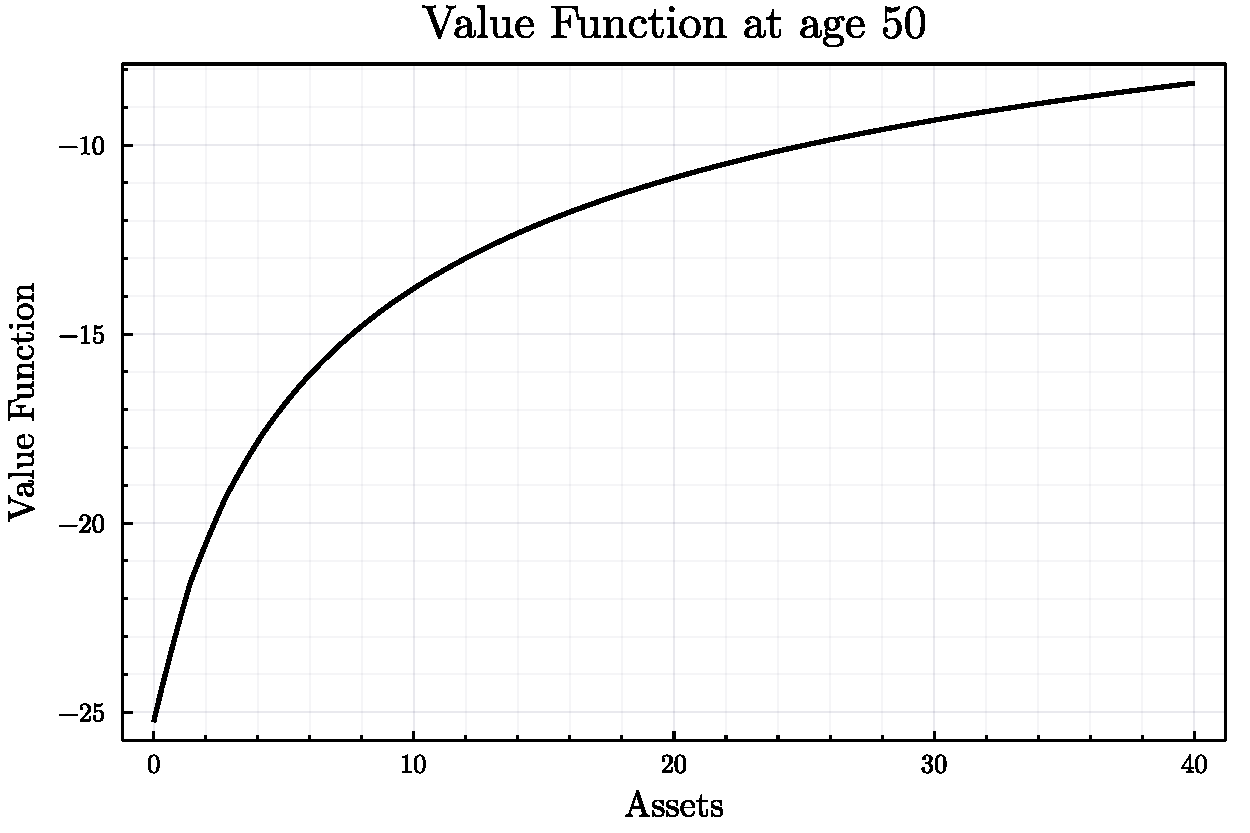
\includegraphics[width=0.7\linewidth]{../Figures/value_function50.pdf}
  \end{center}
  It is increasing and concave.
  
  The savings function for a worker at the model-age 20, $ a'_{20}(z, a) = a'-a $ is the following.
  \begin{center}
    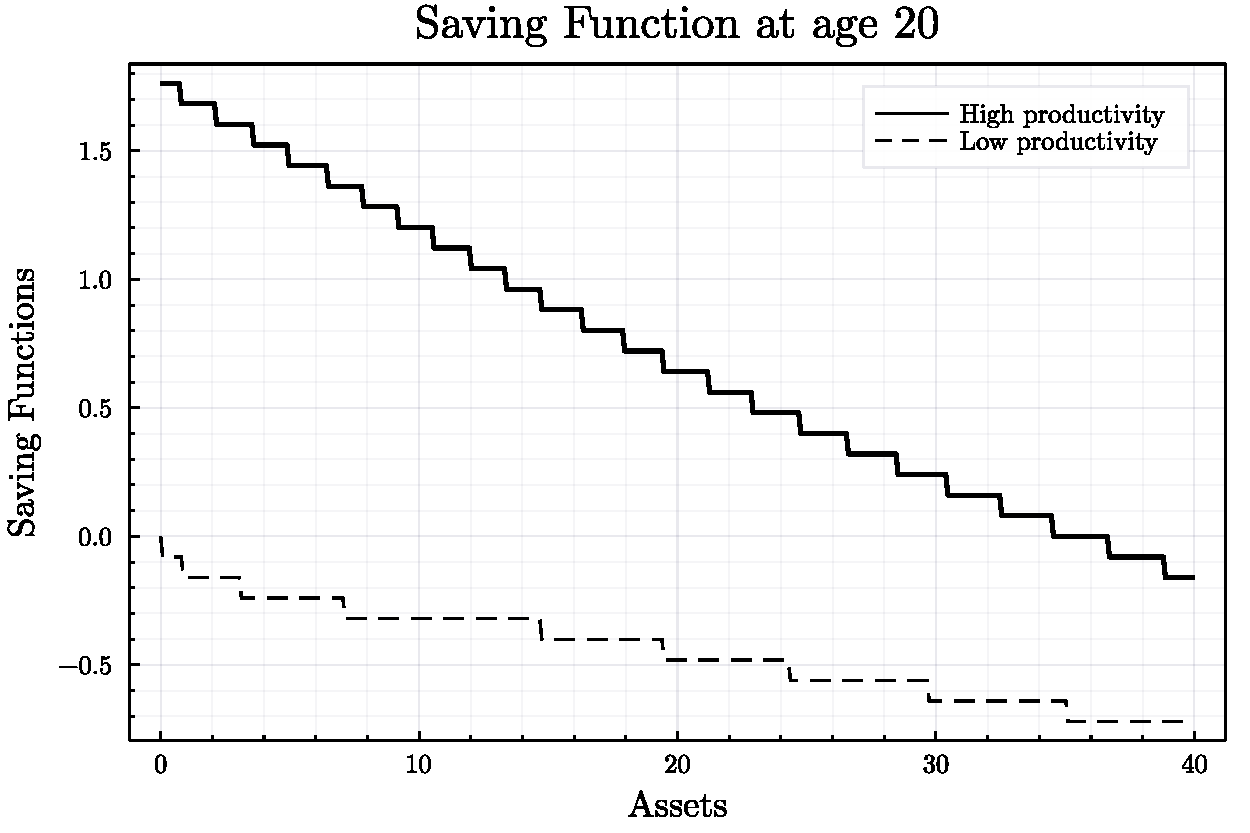
\includegraphics[width=0.7\linewidth]{../Figures/savings_20.pdf}
  \end{center}
  The saving is decreasing in $a$ and increasing in $z$.
\end{solution}

\subsubsection*{Exercise 2}
After solving for agent's dynamic programming problem, solve for the steady-state distribution of agents over age, productivity and asset holdings, $ F_j (z, a) $. Find first the relative sizes of each cohort of age $ j $ (denoted by $ \mu_j $ ) using the expression below: \[ \mu_{i+1} = \frac{\mu_i}{1 +N}, \; \text{for } \; i = 1, \hdots, N-1  \]  with any $ \mu_1 = \tilde{\mu}_1 >0 $. Then normalize $ \mu $, so that it sums up to 1 across all age groups. Finally, start with the newborn generation with zero wealth: given its distribution, $ F_1(z^H, 0) = \mu_1 × 0.2037 $ and $ F_1(z^L, 0) = \mu_1×0.7963 $, compute the distribution of agents over asset holdings at subsequent ages by applying the optimal decision rules.
\begin{solution}
  See the code and report the results in Exercise 3 based on Exercise 2.  
\end{solution}

\subsubsection*{Exercise 3}
\begin{enumerate}
\item First, solve for the benchmark model with social security. Is this economy dynamically efficient (compare the interest rate with the implicit return from social security, which is equal to the population growth rate)? Now eliminate social security by setting $ \theta = 0 $. Observe how aggregate capital accumulation and labor supply change as a result of the tax reform. Provide intuition in terms of insurance and output efficiency. How does aggregate welfare change? Who benefits and who loses due to this reform? How does the reform affect cross-sectional wealth inequality? You can use table 1 to support your answers.
  \begin{solution}
    Table \ref{tab1} summarises the results. This economy is not efficient because it is not equal to population growth. The total welfare decrease. Figure \ref{lambda} shows the effect of this policy change by age. Only a few young gets a benefit. 
  \end{solution}

\item In the second experiment, there is no idiosyncratic risk. Assume that at each age $ j $, $ z^L = z^H = 0.5. $ First, compute the aggregate variables for the case with social security. How does the aggregate capital stock change relative to the benchmark model? Provide intuition in terms of capital as a buffer stock. Then, eliminate social security. How does the aggregate welfare change? What can you conclude about social security as an insurance device against idiosyncratic risk? Comment on the extent, to which these welfare comparisons across steady states are meaningful or misleading.
  \begin{solution}
    The welfare decreases. Social security decreases comparing with the benchmark model. The aggregate capital decreases because people don't have saving demand for the shock. If social security is eliminated, the aggregate welfare does not change well. The result suggests that social security works as insurance because welfare decreases in the benchmark when the social security is removed.     
  \end{solution}
  
\item Consider the case, when labor supply is exogenous $ (\gamma = 1 $). Compare the distortionary effect of social security on the aggregate labor supply. How does the support for social security change with exogenous labor supply?
  \begin{solution}
    Social security does not change the aggregate labor supply even without social security. Without social security, total welfare decreases. So, fewer people support the social security change.  
  \end{solution}
  \begin{table} 
    \centering
    \caption{\label{tab1} Results of policy experiments}
\begin{tabular}{lcccccc}
 \hline
 \hline
 &\multicolumn{2}{c}{Benchmark Model} &\multicolumn{2}{c}{No risk, $z^L=z^H=0.5$}&\multicolumn{2}{c}{Exogenous labor, $\gamma=1$}\\
 \hline
 capital, $K$ & 3.362 & 4.59 & 1.073 & 1.347 & 6.952 & 9.12 \\
 labor, $L$ & 0.343 & 0.365 & 0.162 & 0.174 & 0.754 & 0.754 \\
 wage, $w$ & 1.455 & 1.592 & 1.263 & 1.338 & 1.424 & 1.57 \\
 interest, $r$ & 0.024 & 0.011 & 0.048 & 0.037 & 0.027 & 0.013 \\
 pension benefit, $b$ & 0.225 & 0.0 & 0.092 & 0.0 & 0.484 & 0.0 \\
 total welfare, $W$ & -35.797 & -37.116 & -44.906 & -44.825 & -23.26 & -25.438 \\
 cv(wealth) & \textemdash & -0.195 & \textemdash & -0.087 & \textemdash & -0.194
 \\\hline
 \end{tabular}
  \end{table}
\begin{figure}
\centering
    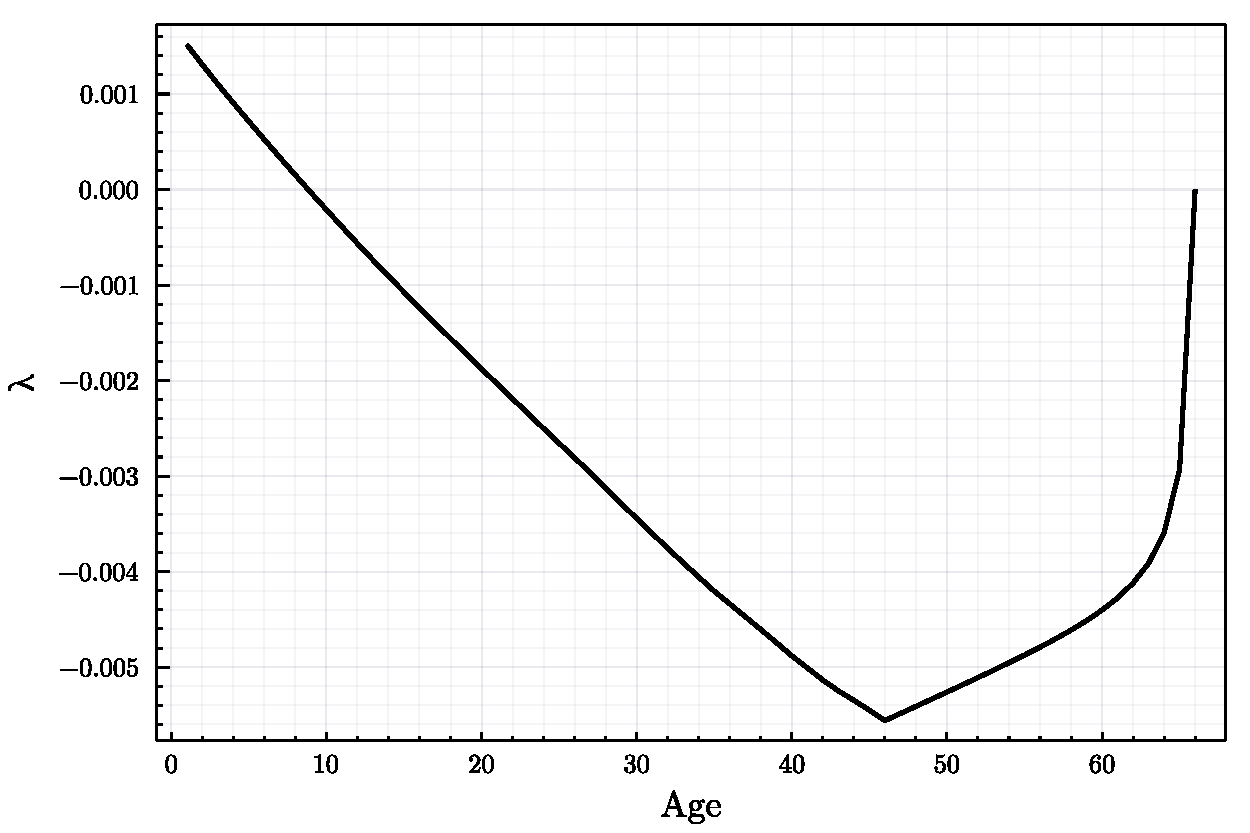
\includegraphics[width=0.7\linewidth]{../Figures/lambda.pdf}
\caption{\label{lambda} Effects of Policy Change by Age}

\end{figure}

\end{enumerate}
\end{document}